\let\negmedspace\undefined
\let\negthickspace\undefined
\documentclass[journal,12pt,twocolumn]{IEEEtran}
\usepackage{cite}
\usepackage{amsmath,amssymb,amsfonts,amsthm}
\usepackage{algorithmic}
\usepackage{graphicx}
\usepackage{textcomp}
\usepackage{xcolor}
\usepackage{txfonts}
\usepackage{listings}
\usepackage{enumitem}
\usepackage{mathtools}
\usepackage{gensymb}
\usepackage{comment}
\usepackage[breaklinks=true]{hyperref}
\usepackage{tkz-euclide} 
\usepackage{listings}
\usepackage{gvv}                                        
\def\inputGnumericTable{}                                 
\usepackage[latin1]{inputenc}                                
\usepackage{color}                                            
\usepackage{array}                                            
\usepackage{longtable}                                       
\usepackage{calc}                                             
\usepackage{multirow}                                         
\usepackage{hhline}                                           
\usepackage{ifthen}                                           
\usepackage{lscape}
\usepackage{enumitem}
\newtheorem{theorem}{Theorem}[section]
\newtheorem{problem}{Problem}
\newtheorem{proposition}{Proposition}[section]
\newtheorem{lemma}{Lemma}[section]
\newtheorem{corollary}[theorem]{Corollary}
\newtheorem{example}{Example}[section]
\newtheorem{definition}[problem]{Definition}
\newcommand{\BEQA}{\begin{eqnarray}}
\newcommand{\EEQA}{\end{eqnarray}}
\newcommand{\define}{\stackrel{\triangle}{=}}
\theoremstyle{remark}
\newtheorem{rem}{Remark}
\begin{document}
\bibliographystyle{IEEEtran}
\vspace{3cm}
\title{GATE BM Q49}
\author{EE23BTECH11027 - K RAHUL$^{*}$% <-this % stops a space
}
\maketitle
\newpage
\bigskip
\renewcommand{\thefigure}{\theenumi}
\renewcommand{\thetable}{\theenumi}
RESULTS: \\
\begin{align}
u\brak{t} \system{L} \frac{1}{s}\\
tu\brak{t} \system{L} \frac{1}{s^2} \label{lap_1}
\end{align}
	
\begin{align}
    f\brak{t} \system{L} F\brak{s}  \implies f\brak{t+a} \system{L} e^{as}F\brak{s} \label{lap_2}
\end{align}\\
\bigskip

QUESTION:\\
The continuous time signal $x\brak{t}$ is described by:
\begin{align}
x\brak{t}=
    \begin{cases}
        1, & \text{if } 0\: {\displaystyle \leq }\:t\:{\displaystyle \leq }\:1\\
        0, & \text{elsewhere}
    \end{cases} 
\end{align}
If $y\brak{t}$ represents $x\brak{t}$ convolved with itself, which of the following options is/are TRUE?
\begin{enumerate}[label = \Alph*]
    \item $y\brak{t}$ = 0 for all $t<0$\\
    \item $y\brak{t}$ = 0 for all $t>1$\\
    \item $y\brak{t}$ = 0 for all $t>3$\\
    \item $\int_{0.1}^{0.75} \frac{dy\brak{t}}{dt}\: \text{dt} \neq 0$
\end{enumerate} \hfill{GATE 2023 BM- Q 49}\\
\bigskip 
\bigskip
SOLUTION:
\begin{table}[ht]
\setlength{\arrayrulewidth}{0.3mm}
\setlength{\tabcolsep}{15pt}
\renewcommand{\arraystretch}{1.5}



\begin{tabular}{ |p{1cm}|p{3cm}|p{1cm}| }
\hline
Symbol & Description\\
\hline
$X\brak{s}$ & Laplace transform of $x\brak{t}$\\
\hline
$Y\brak{s}$ & Laplace transform of $y\brak{t}$ \\
\hline
$u\brak{t-t_0}$ & Unit step function, $u\brak{t-t_0} = 1, t \geq t_0$\\
\hline
\end{tabular}
\caption{Parameters}

\end{table}
\bigskip
\begin{align}
    y\brak{t} &= x\brak{t} * x\brak{t}\\
    Y\brak{s} &= X\brak{s}X\brak{s}\\
    &=\brak{\frac{1-e^{-s}}{s}}^2\\
    &=\frac{1+e^{-2s}-2e^{-s}}{s^2}
\end{align}
Using \eqref{lap_1} and \eqref{lap_2}, 
\begin{align}
    y\brak{t} = tu\brak{t} + \brak{t-2}u\brak{t-2} -2\brak{t-1}u\brak{t-1}
\end{align}
For $t<0$, $u\brak{t}, u\brak{t-1}, u\brak{t-2}$ all are zero, hence $y\brak{t} = 0$. Thus, option A is right.\\

If $1<t<2$, $u\brak{t}$ and $u\brak{t-1}$ are equal to unity while $u\brak{t-2}$ is equal to 0. Thus, $y\brak{t} = 2-t$. Thus, option B is wrong.\\

If $t>3$, $u\brak{t}, u\brak{t-1}, u\brak{t-2}$ are all equal to unity. Thus, $y\brak{t} = 0$. Thus, option C is right.\\

\begin{align}
    \int_{0.1} ^ {0.75} dy\brak{t} &= y\brak{0.75} - y\brak{0.1} \\
    &= 0.75 - 0.1\\
    &= -0.25
\end{align}
Thus, option D is right.\\
\begin{figure}[h]
    %\caption{Stem Plot of $x(n)$ v/s n}
    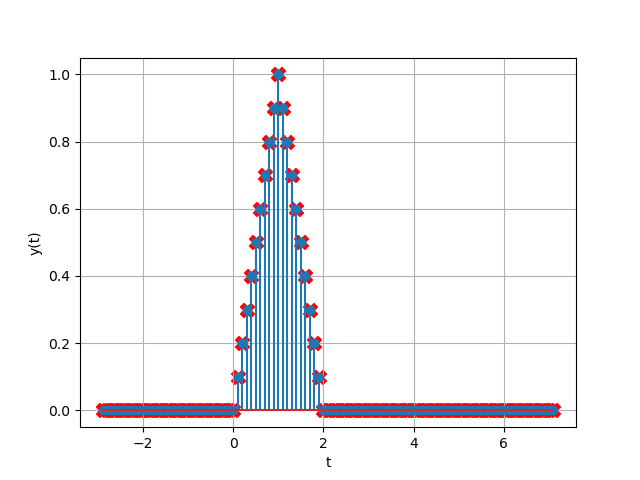
\includegraphics[width=0.3\textwidth]{figs/y(t)_vs_t.png}\label{fig:y(t)_vs_t}
    \caption{Stem Plot of $y(t)$ v/s t}
\end{figure}
\end{document}


